\section{Blockchain Ethereum et smart contracts}
\framewithtitle{Blockchain Ethereum et smart contracts}

\begin{frame}{Sommaire}
  \setcounter{tocdepth}{2}
  \tableofcontents[currentsection, hideothersubsections]
\end{frame}

\begin{frame}{Objectifs de ce module}
  Comprendre les opérations de base de la cryptographie
  \begin{enumerate}
    \item Interagir avec une blockchain de test (Ethereum Sepolia)
    \item Interagir avec une blockchain de production (Polygon)
  \end{enumerate}
\end{frame}

\begin{frame}{Créer un wallet avec MetaMask}
  \begin{columns}
    \begin{column}{0.7\textwidth}
      \begin{itemize}
        \item Ceux qui on déjà un wallet : bonne sieste
        \item Les autres, installez l'extension MetaMask sur votre navigateur (Chrome / Firefox)
        \item Effectuez l'onboarding et notez bien la phrase de récupération
      \end{itemize}
    \end{column}
    \begin{column}{0.25\textwidth}
      \begin{figure}
        \resizebox{\textwidth}{!}{
          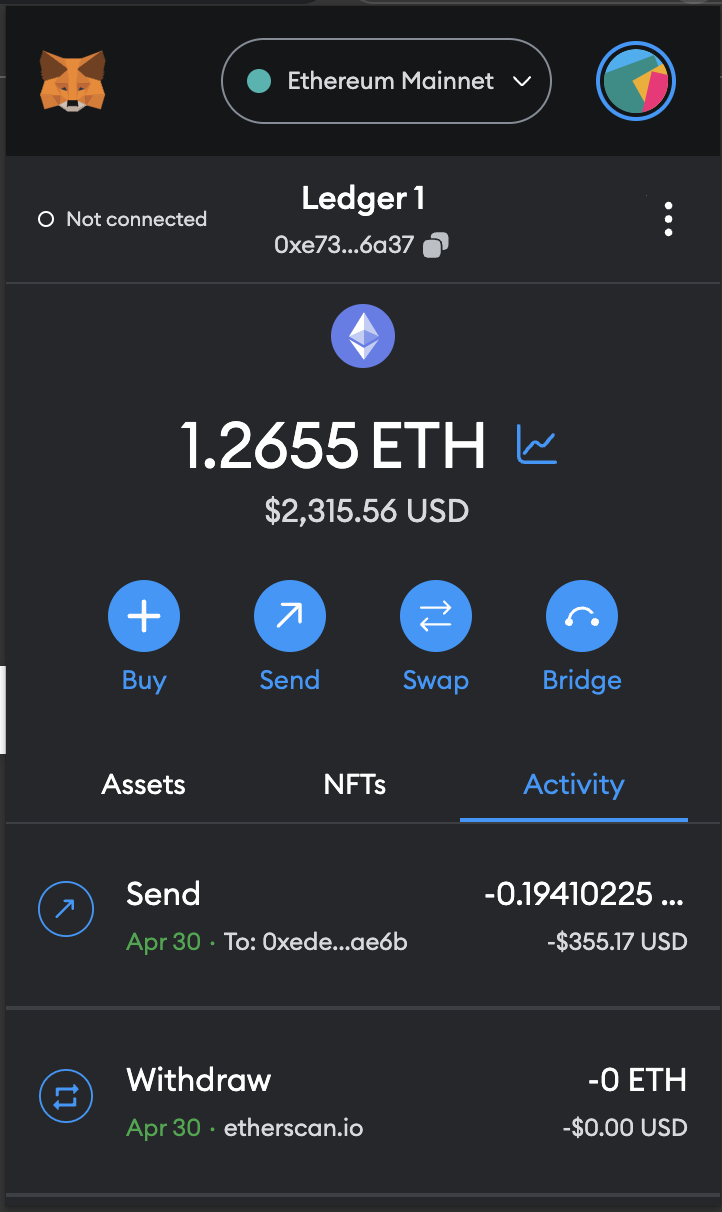
\includegraphics{img/metamask.png}
        }
      \end{figure}
    \end{column}
    \begin{column}{0.05\textwidth}\end{column}
  \end{columns}
\end{frame}

\begin{frame}{Seed phrase}
  Lors de la création d'un wallet avec MetaMask, une phrase de douze mots est générée.

  \begin{center}
    \begin{tcolorbox}[arc=1ex, colback=myuniversity, colframe=myuniversity, left=3pt, right=3pt, top=3pt, bottom=2pt]
      \vspace*{1cm}
      \begin{center}
        \begin{huge}
          \textcolor{white}{
            Il faut absolument la sauvegarder en lieu sûr.\\
            Quiconque l'obtient peut accéder à tout votre wallet, vos cryptos et vos NFTs !
          }
        \end{huge}
      \end{center}
      \vspace*{1cm}
    \end{tcolorbox}
  \end{center}
\end{frame}

\begin{frame}{Notion de gas}
  \begin{itemize}
    \item Contrairement à la blockchain Bitcoin, les frais Ethereum ne paie pas à la transaction mais à la complexité du calcul
    \item Transférer de l'Ether entre deux comptes est beaucoup moins coûteux que faire participer à une enchère de NFTs
    \item La complexité des transactions en Ethereum se mesure en \textquote{gas}
    \item L'utilisateur peut choisir le prix du gas affecté à sa transaction.
    \item Le gas se mesure en Gwei avec 1 ETH = 1000000000 Gwei
  \end{itemize}
\end{frame}
\subsection{Développer des contrats avec Foundry}
\framewithtitle{Foundry}

\begin{frame}{Foundry}
  Dans ce cours, nous allons utiliser Foundry, un utilitaire permettant de développer des smart-contracts simplement.
\end{frame}

\begin{frame}[fragile]{Installation de Foundry : Windows}
  Il faut d'abord installer Windows Subsystem Linux avec :
  \begin{minted}{bash}
    $ wsl --install
  \end{minted}

  WSL demandera de redémarrer, puis au redémarrage de choisir un nom d'utilisateur et un mot de passe.
  Pour confirmer la bonne installation de WSL, exécuter :

  \begin{minted}{bash}
    $ wsl --list
  \end{minted}
\end{frame}

\begin{frame}[fragile]{Installation de Foundry}
  Configurer git avec votre nom / email :

  \begin{minted}{bash}
    $ git config --global user.email "you@example.com"
    $ git config --global user.name "Prénom Nom"
  \end{minted}

  Installer Foundryup (installateur de Foundry)
  \begin{minted}{bash}
    $ curl -L https://foundry.paradigm.xyz | bash
  \end{minted}

  Redémarrer le terminal, lancer Foundryup
  \begin{minted}{text}
    $ foundryup
  \end{minted}

  Redémarrer le terminal, lancer Forge
  \begin{minted}{text}
    $ forge
    forge 0.2.0 (31fcf5a 2023-05-19T00:10:33.861185000Z)
  \end{minted}
\end{frame}

\begin{frame}{Architecture d'un projet Foundry}
  \dirtree{%
    .1 /.
    .2 out\DTcomment{Fichiers compilés}.
    .2 lib\DTcomment{Libraries installées}.
    .2 src\DTcomment{Code source des contrats}.
    .2 test\DTcomment{Test des contrats}.
    .2 .gitmodules.
    .2 foundry.toml\DTcomment{Configuration de Foundry}.
  }
\end{frame}
\framewithtitle{Solidity}

\begin{frame}{Qu'est-ce qu'un smart contract}
  \begin{block}{Définition : smart contract}
    Sur la blockchain Ethereum, un smart contract est un bytecode (=code hexadécimal) associé à une adresse.

    $\Rightarrow$ Les adresses des smart contracts sont indiscernables des adresses des comptes utilisateurs.
  \end{block}

  \begin{block}{Définition : Externally Owned Account}
    Les adresses contrôlés par des utilisateurs sont appelées \enquote{Externally Owned Account} (EOA).
  \end{block}

  Voir le glossaire d'Ethereum: \url{https://ethereum.org/en/glossary}
\end{frame}

\begin{frame}{Solidity ?}
  \begin{block}{Définition : Solidity}
    Solidity est un \textbf{langage de programmation} utilisé pour écrire des smart contracts sur la plateforme Ethereum.

    Solidity permet aux développeurs de définir des règles et des logiques spécifiques à un smart contract.
    Il permet d'écrire des lignes de code qui définissent comment un smart contract doit fonctionner, quelles actions il doit effectuer et comment il doit réagir dans différentes situations.

    En utilisant Solidity, les développeurs peuvent créer des smart contracts pour diverses applications décentralisées (dApps)
  \end{block}
\end{frame}

\begin{frame}[fragile]{Solidity : syntaxe en POO}
  \begin{minted}{solidity}
    // SPDX-License-Identifier: UNLICENSED
    pragma solidity ^0.8.13;
    
    contract Counter {
        uint256 public number;
    
        function setNumber(uint256 newNumber) public {
            number = newNumber;
        }
    }
  \end{minted}
\end{frame}

\begin{frame}[fragile]{Solidity : header}
  Le header d'un smart contract s'écrit en deux lignes :

  \begin{minted}{solidity}
    // SPDX-License-Identifier: UNLICENSED
    pragma solidity ^0.8.13;
  \end{minted}

  La ligne 1 défini la licence du fichier :

  \begin{itemize}
    \item \solidity{UNLICENSED} signifie que le code est complètement privé
    \item \solidity{pragma solidity ^0.8.13;} version de Solidity compatible avec le fichier
  \end{itemize}
\end{frame}

\begin{frame}{Semantic versionning}
  \begin{block}{Semantic versionning \enquote{SemVer}}
    Le versionnage sémantique  est une méthode de numérotation des versions logicielles basée sur des règles spécifiques.
    Elle se compose de trois nombres séparés par des points : MAJEUR.MINEUR.PATCH.
    Le numéro MAJEUR est augmenté lorsque des changements incompatibles sont apportés, le numéro MINEUR est augmenté lorsque des fonctionnalités sont ajoutées de manière rétrocompatible, et le numéro PATCH est augmenté pour les corrections de bugs rétrocompatibles.
  \end{block}

  \begin{columns}
    \begin{column}{0.48\textwidth}
      \begin{block}{Opérateurs}
        \begin{itemize}
          \item \texttt{=1.2.3} strictement égal à 1.2.3
          \item \texttt{\^{}1.2.3} $\Rightarrow$ \texttt{1.2.3 < v < 2.0.0}
          \item \texttt{\~{}1.2.3} $\Rightarrow$ \texttt{1.2.3 < v < 1.3.0}
        \end{itemize}
      \end{block}
    \end{column}
    \hspace{0.01\textwidth}
    \begin{column}{0.48\textwidth}
      \begin{block}{Opérateurs (MAJEUR=0)}
        \begin{itemize}
          \item \texttt{=0.1.2} strictement égal à 0.1.2
          \item \texttt{\^{}0.1.2} $\Rightarrow$ \texttt{0.1.2 < v < 0.2.0}
        \end{itemize}

        \vspace{1em}
        \vspace{\smallskipamount}
      \end{block}
    \end{column}
  \end{columns}
\end{frame}

\begin{frame}{Solidity : types primitifs}
  \begin{itemize}
    \item \solidity{uint} un entier non signé sur 256 bits
    \item \solidity{uint8} un entier non signé sur 8 bits
    \item \solidity{uint32} un entier non signé sur 32 bits
    \item \solidity{uint256} un entier non signé sur 256 bits
    \item \solidity{int} un entier signé sur 256 bits
    \item \solidity{int32} un entier signé sur 32 bits
    \item \solidity{address} une adresse Ethereum
    \item \solidity{string} une chaîne de caractères
    \item \solidity{struct} structure, au sens langage C du terme
    \item \solidity{mapping} une association clé-valeur
  \end{itemize}
\end{frame}

\begin{frame}[fragile]{Solidity : le type \texttt{address}}
  Le type \solidity{address} est spécial et possède des propriétés :

  \begin{itemize}
    \item \solidity{<address>.balance} le montant d'ether détenu par l'adresse
    \item \solidity{<address>.code} le code à l'adresse (vide pour les EOA)
    \item Dans un contrat, \solidity{address(this).balance} donne la balance du contrat
  \end{itemize}
\end{frame}

\begin{frame}{Solidity : variables spéciales}
  \begin{block}{\texttt{msg} (= message)}
    Un message représente un appel d'une fonction d'un smart contract.

    \begin{itemize}
      \item \solidity{msg.sender} expéditeur du message
      \item \solidity{msg.value} nombre d'Ether envoyés avec le message
    \end{itemize}
  \end{block}


  \begin{block}{\texttt{block}}
    Metadata du bloc actuel.

    \begin{itemize}
      \item \solidity{block.number} numéro du bloc actuel
      \item \solidity{block.timestamp} tinmestamp UNIX en secondes
    \end{itemize}
  \end{block}
\end{frame}

\begin{frame}[fragile]{Solidity : contrôle de flow}
  \begin{columns}
    \begin{column}{0.47\textwidth}
      \solidity{if} / \solidity{else} / \solidity{else if}

      \begin{minted}{solidity}
        if (cond) {
          // if path
        } else if (cond2) {
          // else if path
        } else {
          // else path
        }
      \end{minted}

      Note : pas de \solidity{switch / case} en Solidity.
    \end{column}
    \vspace{0.03\textwidth}
    \begin{column}{0.47\textwidth}
      \solidity{for} / \solidity{while}

      \begin{minted}{solidity}
        for (uint256 i = 0; i < n; i++) {
          // do stuff
        }

        while(cond) {
          // do other stuff
        }
      \end{minted}

      Note : pas de \solidity{do while} en Solidity.
    \end{column}
  \end{columns}
\end{frame}

\begin{frame}[fragile]{Solidity : visibilité}
  \begin{columns}
    \begin{column}{0.47\textwidth}
      \begin{block}{Public}
        \begin{minted}{solidity}
          uint public myVariable;
          function myFunction() public {
            // Function logic
          }
        \end{minted}
      \end{block}
    \end{column}
    \vspace{0.03\textwidth}
    \begin{column}{0.47\textwidth}
      \begin{block}{Private}
        \begin{minted}{solidity}
          uint internal myVariable;
          function myFunction() internal {
            // Function logic
          }
        \end{minted}
      \end{block}
    \end{column}
  \end{columns}

  \begin{columns}
    \begin{column}{0.47\textwidth}
      \begin{block}{Internal}
        \begin{minted}{solidity}
          uint internal myVariable;
          function myFunction() internal {
            // Function logic
          }
        \end{minted}
      \end{block}
    \end{column}
    \vspace{0.03\textwidth}
    \begin{column}{0.47\textwidth}
      \begin{block}{External}
        \begin{minted}{solidity}
          // external variables not possible 
          function myFunction() external {
            // Function logic
          }
        \end{minted}
      \end{block}
    \end{column}
  \end{columns}
\end{frame}

\begin{frame}[fragile]{Solidity : \texttt{modifier}}
  \begin{block}{Définition : \texttt{modifier}}
    En Solidity, un \enquote{modifier} est une fonction spéciale qui permet de modifier le comportement d'autres fonctions dans un contrat intelligent.
    Les modifiers fournissent un moyen pratique de réutiliser du code et d'ajouter des conditions supplémentaires ou des vérifications avant l'exécution d'une fonction.
  \end{block}


  \begin{block}{Syntaxe : \texttt{modifier}}
    \begin{minted}{solidity}
    modifier exampleModifier() {
      _; // Continue function execution
    }

    function foobar() public exampleModifier {}
  \end{minted}
  \end{block}
\end{frame}

\begin{frame}[fragile]{Solidity : interfaces}
  Comme beaucoup d'autres langages, Solidity dispose d'interfaces\footnote{Voir la \href{https://docs.soliditylang.org/fr/stable/contracts.html\#interfaces}{documentation Solidity des interfaces}} qui servent à intégrer des notions de polymorphisme.

  \begin{itemize}
    \item Elles ne peuvent pas hériter d'autres contrats, mais elles peuvent hériter d'autres interfaces.
    \item Toutes les fonctions déclarées doivent être externes.
    \item Elles ne peuvent pas déclarer de \texttt{constructor}, de variables d'état ou de \texttt{modifier}.
  \end{itemize}

  \begin{block}{Syntaxe : interface}
    \begin{minted}{solidity}
      interface IIoken {
        function transfer(address recipient, uint amount) external;
      }
    \end{minted}
  \end{block}
\end{frame}

\begin{frame}[fragile]{Solidity : events}
  \begin{itemize}
    \item La blockchain est \enquote{isolée} du monde extérieur : impossible de contacter le monde extérieur (pas de requête HTTP, notifications, etc.).
    \item Solidity permet de définir des events qui peuvent être écoutés à l'extérieur de la blockchain.
  \end{itemize}

  \begin{minted}{solidity}
    // Event declaration
    event Minted(address indexed to, uint256 amount);

    function transfer(address to, uint256 amount) {
      balanceOf[to] += amount;
      emit Minted(to, value); // Event emission
    }
  \end{minted}

  \begin{minted}{typescript}
    client.watchEvent({
      address: '0xa0b86991c6218b36c1d19d4a2e9eb0ce3606eb48',
      event: parseAbiItem('event Minted(address indexed to, uint256 amount)'), 
      onLogs: logs => console.log(logs)
    })
  \end{minted}
\end{frame}

\begin{frame}[fragile]{Solidity : events indexed}
  Les events peuvent avoir certains de leurs arguments marqués comme \solidity{indexed}.
  Cela permet de filtrer sur les valeurs ces arguments.

  Exemple : \solidity{event Transfer(address indexed from, address indexed to, uint256 value)}.

  \begin{itemize}
    \item Si on considère deux addresses \texttt{x} et \texttt{y}:
    \item Il est possible d'écouter les transactions émises par \texttt{x}
    \item Il est possible d'écouter les transactions reçues par \texttt{x}
    \item Il est possible d'écouter les transactions émises par \texttt{x} vers \texttt{y}
    \item Il n'est pas possible d'écouter les transactions de 1 ETH ou moins car \solidity{uint256 value} n'est pas \solidity{indexed}.

  \end{itemize}
\end{frame}

\begin{frame}[fragile]{Solidity : erreurs}
  Souvent, il faut arrêter l'exécition d'un smart contract et renvoyer une erreur (exécution non autorisée, opération impossible, etc.).

  \begin{columns}
    \begin{column}{0.47\textwidth}
      Fonction \solidity{revert(bool assertion, string message)}

      Revert si \solidity{assertion} est évalué à false.
    \end{column}
    \vspace{0.01\textwidth}
    \begin{column}{0.47\textwidth}
      Custom errors: permet de déclarer des erreurs avec des paramètres.

      \begin{minted}{solidity}
        contract Foo {
          error Custom(uint256 arg1);

          function willRevert() public {
            revert Custom(1);
          }
        }
      \end{minted}
    \end{column}
  \end{columns}
\end{frame}

\begin{frame}[fragile]{Exemple : cryptomonnaie avec mint initial}
  \begin{minted}{solidity}
    contract Mewo {
      uint256 constant MAX_SUPPLY = 1000000000; // 1 billion
      mapping(address => uint256) public balances;

      contructor() {
        balances[msg.sender] += MAX_SUPPLY; // Initial mint
      }

      function transfer(address to, uint256 amount) public {
        require(balances[msg.sender] >= amount, "Insufficient balance");
        balances[msg.sender] -= amount;
        balances[to] += amount;
      }
    }
  \end{minted}
\end{frame}

\begin{frame}[fragile]{Exemple : cryptomonnaie}
  \begin{minted}{solidity}
    contract Mewo {
      mapping(address => uint256) public balances;

      function transfer(address to, uint256 amount) public {
        require(balances[msg.sender] >= amount, "Insufficient balance");
        balances[msg.sender] -= amount;
        balances[to] += amount;
      }
    }
  \end{minted}
\end{frame}

\begin{frame}[fragile]{Exemple : cryptomonnaie avec mint}
  \begin{minted}{solidity}
    contract Mewo {
      mapping(address => uint256) public balances;

      function mint(uint256 amount) public {
        balances[msg.sender] += amount
      }

      function transfer(address to, uint256 amount) public {
        require(balances[msg.sender] >= amount, "Insufficient balance");
        balances[msg.sender] -= amount;
        balances[to] += amount;
      }
    }
  \end{minted}
\end{frame}

\begin{frame}[fragile]{Exemple : cryptomonnaie avec mint protégé}
  \begin{minted}{solidity}
    contract Mewo {
      address owner;
      mapping(address => uint256) public balances;

      constructor() {
          owner = msg.sender;
      }
    
      modifier onlyOwner() {
          require(msg.sender == owner, "Only owner");
          _;
      }
    
      function mint(uint256 amount) public onlyOwner {
          balances[msg.sender] += amount;
      }
    }
  \end{minted}
\end{frame}

\begin{frame}{Notion de gas}
  \begin{itemize}
    \item Les frais Ethereum ne paie pas à la transaction mais à la \textbf{complexité du calcul}
    \item Transférer de l'Ether entre deux comptes est beaucoup moins coûteux que faire participer à une enchère de NFTs
    \item La complexité des transactions en Ethereum se mesure en \enquote{gas}
    \item Le prix d'un \enquote{gas} se mesure en Gwei avec 1 ETH = 1000000000 Gwei.
    \item L'utilisateur peut choisir le prix du \enquote{gas} affecté à sa transaction.
  \end{itemize}

  \begin{block}{Exemple : \texttt{Mewo.mint}}
    \begin{itemize}
      \item Gas utilisé pour la fonction mint : $24634$
      \item Prix du gas : $37$ gwei/gas
      \item Prix d'un ETH = \$1,817.85
      \item Total = $24634\times37=911458$ gwei $= 0.000911458$ ETH $ = \$1.657$
    \end{itemize}
  \end{block}
\end{frame}

\framewithtitle{Tokens Standards}

\begin{frame}{Qu'est-ce qu'un token ?}
  \begin{block}{Définition : token}
    Dans le contexte de la blockchain Ethereum, un "token" fait référence à une unité de valeur numérique qui est émise et utilisée sur le réseau Ethereum.
  \end{block}

  \begin{itemize}
    \item La création d'un token sur Ethereum est réalisée en mettant en place un smart contract qui définit les règles et les fonctionnalités spécifiques du token.
    \item Ce smart contract est ensuite déployé sur la blockchain Ethereum, ce qui lui permet d'interagir avec d'autres contrats et d'être utilisé par les utilisateurs du réseau.
    \item Les tokens sur Ethereum peuvent être transférés entre différentes adresses Ethereum, ce qui permet des transactions peer-to-peer.
  \end{itemize}
\end{frame}

\begin{frame}{ERC-20 : besoin de standardisation}
  \begin{itemize}
    \item Le standard ERC-20 a été créé dans le but de faciliter l'émission et l'interopérabilité des tokens sur la blockchain Ethereum.
    \item Avant l'introduction du standard ERC-20, chaque token avait son propre smart contract avec des règles et des interfaces spécifiques, ce qui rendait difficile l'interaction entre les tokens et leur intégration dans des applications tierces.
    \item Le standard ERC-20 définit \textbf{une interface} que doivent suivre les contrats qui l'implémentent.
    \item Grâce à cette norme, les tokens ERC-20 peuvent être facilement créés, gérés, échangés et utilisés par les utilisateurs, les portefeuilles et les plateformes d'échange.
  \end{itemize}
\end{frame}

\begin{frame}{ERC-20 : tokens fongibles}
  Le standard ERC-20 défini les tokens \enquote{fongibles}.

  \begin{block}{Définition : token fongible}
    Un token fongible est un type de token dans lequel chaque unité est interchangeable avec une autre unité du même type.
    Cela signifie que chaque token fongible est considéré comme équivalent et peut être remplacé par un autre token identique, sans qu'il y ait de distinction ou de différence entre eux.
  \end{block}

  \begin{itemize}
    \item C'est la perception \enquote{naturelle} de la monnaie : un billet de 5 euros a exactement la même valeur qu'un autre billet de 5 euros.
    \item Chaque unité d'un token fongible ERC-20 est identique en termes de valeur, de fonctionnalité et de propriétés.
  \end{itemize}
\end{frame}

\begin{frame}[fragile]{ERC-20 : interface}
  \begin{minted}{solidity}
    interface IERC20 {
      function name() public view returns (string)
      function symbol() public view returns (string)
      function decimals() public view returns (uint8)
      function totalSupply() public view returns (uint256)
      function balanceOf(address _owner) public view returns (uint256 balance)
      function transfer(address _to, uint256 _value) public returns (bool success)
      function transferFrom(address _from, address _to, uint256 _value) public returns (bool success)
      function approve(address _spender, uint256 _value) public returns (bool success)
      function allowance(address _owner, address _spender) public view returns (uint256 remaining)

      event Transfer(address indexed _from, address indexed _to, uint256 _value)
      event Approval(address indexed _owner, address indexed _spender, uint256 _value)
    }
  \end{minted}
\end{frame}

\begin{frame}[fragile]{ERC-20 : metadata}
  Le nom et le symbole d'un token ERC-20 sont encodés dans le contrat avec les fonctions \solidity{name} et \solidity{symbol}.

  \begin{minted}{solidity}
    contract ERC20 {
      function name() public view returns (string) {
        return "MyToken";
      }

      function symbol() public view returns (string) {
        return "MYT";
      }
    }
  \end{minted}
\end{frame}

\begin{frame}[fragile]{ERC-20 : decimals}
  Solidity ne supporte pas les nombres flottants donc il n'est a priori pas possible d'échanger 0.5 MYT. La technique consiste à considérer que :

  $$1\text{MYT} = 1\underbrace{000000000000000000}_\text{decimals = 18}$$

  \begin{minted}{solidity}
    contract ERC20 {
      function decimals() public view returns (uint8) {
        return 18;
      }
    }
  \end{minted}
\end{frame}

\begin{frame}[fragile]{ERC-20 : \texttt{transfer} de tokens}
  \begin{itemize}
    \item Le nombre de tokens détenus par une adresse s'obtient avec la fonction \solidity{balanceOf}.
    \item Une adresse peut envoyer des tokens à une autre adresse avec la fonction \solidity{function transfer(address to, uint256 amount)}. Contraintes :\begin{itemize}
            \item \solidity{to} ne peut pas être l'adresse zéro
            \item \solidity{msg.sender} doit posséder au moins \solidity{amount} tokens
          \end{itemize}
  \end{itemize}
\end{frame}

\begin{frame}[fragile]{ERC-20 : \texttt{transferFrom}}
  Intégrer les tokens ERC-20 avec d'autres smart contracts nécessite de pouvoir transférer au nom de l'utilisateur.

  Cela permet notamment d'intégrer des fonctionnalités du type \enquote{envoyez des tokens et pourrez faire la chose X}.

  Exemple : envoyez 1 USDC et receivez 5 MYT.

  \begin{minted}{solidity}
    contract Sale {
      MyToken myt;
      ERC20 usdc;

      function buy(uint256 amount) public {
        usdc.transferFrom(msg.sender, address(this), amount);
        myt.mint(address(this), amount);
      }
    }
  \end{minted}
\end{frame}

\begin{frame}[fragile]{ERC-20 : \texttt{allowance}}
  Problème : il faut protéger la fonction \solidity{function transferFrom}

  \begin{block}{Définition : allowance}
    Dans le contexte du standard ERC-20, \textbf{allowance} fait référence à une fonctionnalité qui permet à une adresse Ethereum spécifique d'accéder à un certain nombre de tokens détenus par une autre adresse Ethereum et de les transférer ultérieurement.

    L'allowance est souvent utilisée dans le cadre des transferts de tokens ERC-20 à des tiers de confiance, tels que des contrats ou des dApps (applications décentralisées).
    Elle permet à un propriétaire de tokens de définir une autorisation spécifique pour un dépensier donné.
    Cette autorisation est enregistrée dans le smart contract du token ERC-20.
  \end{block}
\end{frame}

\begin{frame}[fragile]{ERC-20 : \texttt{allowance}}
  \begin{columns}
    \begin{column}{0.4\textwidth}
      La fonction \solidity{approve} permet de définir l'\solidity{allowance} d'une adresse Ethereum.

      Reprenons le contrat \texttt{Sale} avec les contrats :

      \begin{itemize}
        \item Bob, notre utilisateur
        \item \texttt{USDC}, un stablecoin
        \item \texttt{MyToken}, notre token ERC20
        \item \texttt{Sale}, qui vend des MYT contre des USDC
      \end{itemize}

      Nous allons analyser l'utilisation de l'allowance par Bob.
    \end{column}

    \begin{column}{0.57\textwidth}
      Situation initiale (\solidity{msg.sender = address(Bob)}):

      \begin{itemize}
        \item \solidity{USDC.balanceOf(address(Bob)) = 10000}
        \item \solidity{USDC.allowance(address(Sale)) = 0}
        \item \solidity{MyToken.balanceOf(address(Bob)) = 0}
      \end{itemize}

      Bob envoie \solidity{USDC.approve(address(Sale), 2000)}
      \begin{itemize}
        \item \solidity{USDC.allowance(address(Sale)) = 2000}
      \end{itemize}

      Bob envoie \solidity{Sale.buy(1000)}
      \begin{itemize}
        \item \solidity{USDC.balanceOf(address(Bob)) = 9000}
        \item \solidity{USDC.allowance(address(Sale)) = 1000}
        \item \solidity{MyToken.balanceOf(address(Bob)) = 5000}
      \end{itemize}
    \end{column}
  \end{columns}
\end{frame}

\begin{frame}[fragile]{ERC-20 : \texttt{increaseAllowance} / \texttt{decreaseAllowance}}
  En plus de la fonction \solidity{approve} certaines implémentations exposent des fonction non-standard permettant de contrôller plus finement l'\solidity{allowance}.,
  \begin{itemize}
    \item \solidity{increaseAllowance} qui correspond à l'opération \solidity{allowance[spender] += amount}
    \item \solidity{decreaseAllowance} qui correspond à l'opération \solidity{allowance[spender] -= amount}
  \end{itemize}

  Ces deux fonctions sont notamment présentent dans l'implémentation d'OpenZeppelin.
\end{frame}

\begin{frame}[fragile]{ERC-20 : avec OpenZeppelin}
  \begin{columns}
    \begin{column}{0.47\textwidth}
      \begin{center}

        \resizebox{0.5\textwidth}{!}{
          
\includegraphics{img/openzeppelin.png}
        }
      \end{center}

      OpenZeppelin est une bibliothèque de smart-contracts contenant notamment une implémentation du standard ERC-20.

      \begin{itemize}
        \item GitHub : \href{https://github.com/OpenZeppelin/openzeppelin-contracts}{OpenZeppelin/openzeppelin-contracts}
        \item Installer : \mintinline{bash}{forge install openzeppelin/openzeppelin-contracts}
      \end{itemize}
    \end{column}

    \hspace{0.03\textwidth}

    \begin{column}{0.47\textwidth}
      \begin{minted}{solidity}
        import { ERC20 } from "openzeppelin";
  
        contract MyToken is ERC20 {
          constructor() ERC20("MyToken", "MYT") {
            _mint(msg.sender, 1000000000e18);
          }
        }
      \end{minted}

      $\Rightarrow$ c'est tout ! À vous de décider des fonctionnalités de votre token ERC-20 !
    \end{column}
  \end{columns}
\end{frame}

\begin{frame}{ERC-721}
  Le standard ERC-721 défini les tokens \enquote{non-fongibles}, appelées \enquote{Non-Fungible Tokens}.

  \begin{block}{Définition : token non fongible (NFT)}
    Un token non fongible (NFT) est un type de token unique et indivisible sur une blockchain. Chaque NFT est distinct et possède des caractéristiques qui le rendent unique.

    \begin{itemize}
      \item Les NFTs tirent leur valeur de leur unicité, de leur rareté et de leur authenticité, ce qui les rend particulièrement adaptés à la représentation d'actifs numériques uniques et à leur propriété vérifiable sur la blockchain.
      \item Chaque NFT possède un identifiant unique qui le distingue des autres tokens, et ses propriétés et sa provenance sont enregistrées dans le registre immuable de la blockchain.
    \end{itemize}
  \end{block}

  Exemple hors blockchain : certaines anciennes pièces de monnaies valent plus que leur valeur faciale (numismatique).
\end{frame}

\begin{frame}[fragile]{ERC-721 interface}
  \begin{minted}{solidity}
    interface ERC721 {
      function balanceOf(address _owner) external view returns (uint256);
      function ownerOf(uint256 _tokenId) external view returns (address);
      function safeTransferFrom(address _from, address _to, uint256 _tokenId, bytes data) external payable;
      function safeTransferFrom(address _from, address _to, uint256 _tokenId) external payable;
      function transferFrom(address _from, address _to, uint256 _tokenId) external payable;
      function approve(address _approved, uint256 _tokenId) external payable;
      function setApprovalForAll(address _operator, bool _approved) external;
      function getApproved(uint256 _tokenId) external view returns (address);
      function isApprovedForAll(address _owner, address _operator) external view returns (bool);
    }
  \end{minted}
\end{frame}

\begin{frame}{ERC-1155}

\end{frame}
\framewithtitle{Tester avec Foundry}

\begin{frame}{Tester un contrat ?}
  Pourquoi ?

  \begin{itemize}
    \item Les contrats sont des programmes exposés aux utilisateurs finaux $\Rightarrow$ un bug peut engendrer \textbf{une perte financière} pour l'utilisateur
    \item Les contrats sont immutables = une fois déployés, il ne peuvent être modifiés
    \item En gros, les contrats doivent être \textbf{parfaits du premier coup}.
  \end{itemize}

  Comment ?

  \begin{enumerate}
    \item Imaginer et créer un scénario (cela revient à définir les variables d'état d'un contrat)
    \item Exécuter la ou les transactions à tester
    \item Vérifier que le nouvel état correspond à celui attendu.
  \end{enumerate}
\end{frame}

\begin{frame}[fragile]{Exemple : Ownable}
  \begin{columns}
    \begin{column}{0.47\textwidth}
      \begin{minted}{solidity}
        contract Ownable {
          address public owner;
    
          modifier onlyOwner() {
            require(msg.sender == owner);
          }
    
          function transferOwnership(address _owner) onlyOwner {
            owner = _owner;
          }
        }      
      \end{minted}
    \end{column}

    \begin{column}{0.47\textwidth}
      Tester la fonction \solidity{transferOwnership}, c'est :

      \begin{enumerate}
        \item \solidity{transferOwnership} renvoie une erreur si \solidity{msg.sender} n'est pas l'\solidity{owner}
        \item \solidity{transferOwnership} ne renvoie pas d'erreur si \solidity{msg.sender} est l'\solidity{owner} et que le nouvel \solidity{owner} est \solidity{msg.sender}
      \end{enumerate}
    \end{column}
  \end{columns}
\end{frame}

\begin{frame}[fragile]{Foundry : créer un test}
  \begin{itemize}
    \item Dans Foundry, les tests s'écrivent en Solidity.
    \item Par convention, on teste le fichier \texttt{Contract.sol} dans \texttt{Contract.\textbf{t}.sol}
    \item Deux méthodes possibles pour placer les tests :
          \begin{itemize}
            \item juste à côté du fichier source
            \item dans le dossier \texttt{test}
          \end{itemize}
  \end{itemize}
\end{frame}

\begin{frame}[fragile]{Foundry : cheat codes}
  Les cheatcodes permettent d'effectuer des actions normalement impossibles dans la blockchain.
  Voici les principaux :

  \begin{itemize}
    \item \solidity{hoax(address who)} le prochain call sera fait en tant que \solidity{who}
    \item \solidity{hoax(address who, uint256 amount)} le prochain call sera fait en tant que \solidity{who} et sa balance en ether sera de \solidity{amount}
    \item \solidity{deal(address who, uint256 amount)} change la balance de \solidity{who} en \solidity{amount}
  \end{itemize}
\end{frame}